
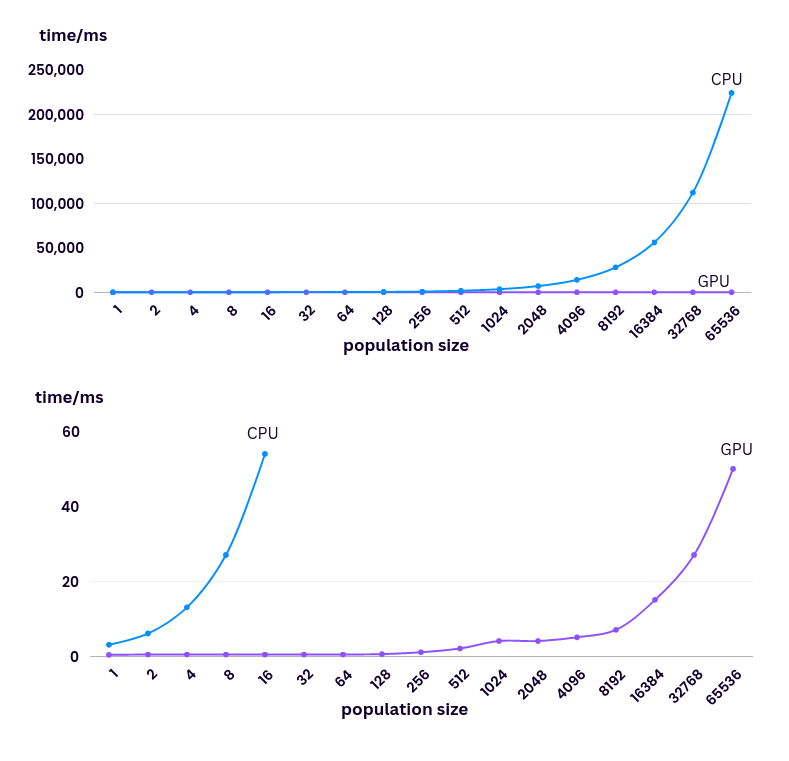
\includegraphics[width=3in]{popsizetime.png}
\caption{3D cube in x, y, z axis}
\label{fig:my_label}
GPU vs CPU time per 1 episode step for different population sizes. GPU is running a program written in GLSL and CPU in Python. It can be seen that the CPU time grows much more quickly.


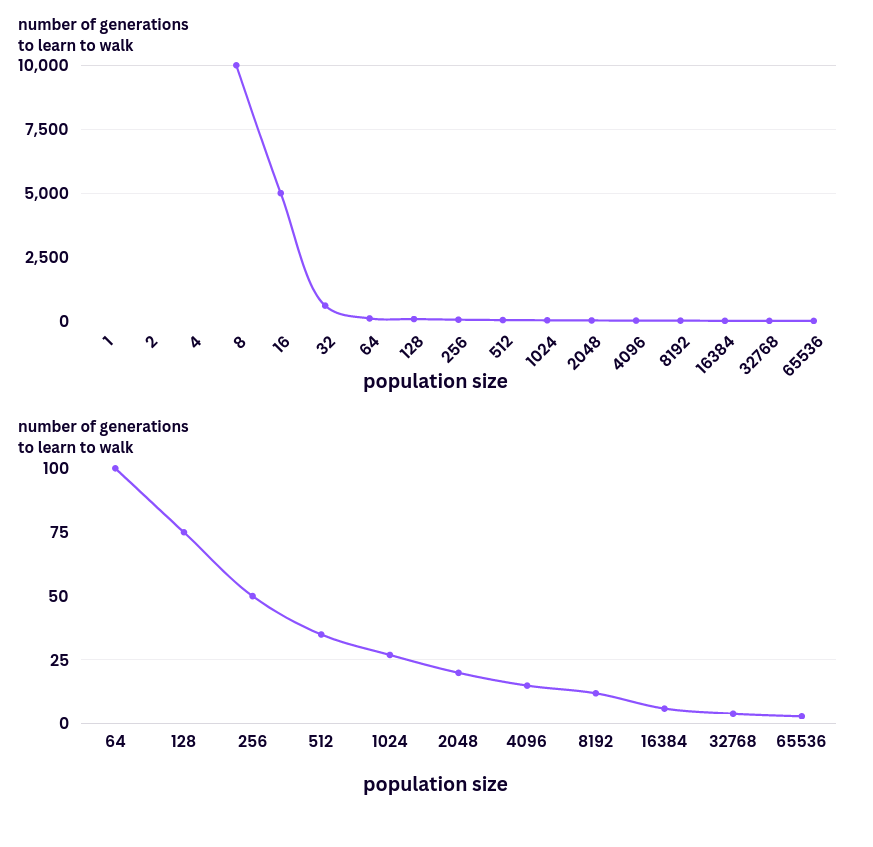
\includegraphics[width=3in]{numberofgenerationstolearntowalk.png}
As the population size grows number of generations to learn to walk falls. This is because when the population size is large, the probability that any creature is walking by pure chance is high.

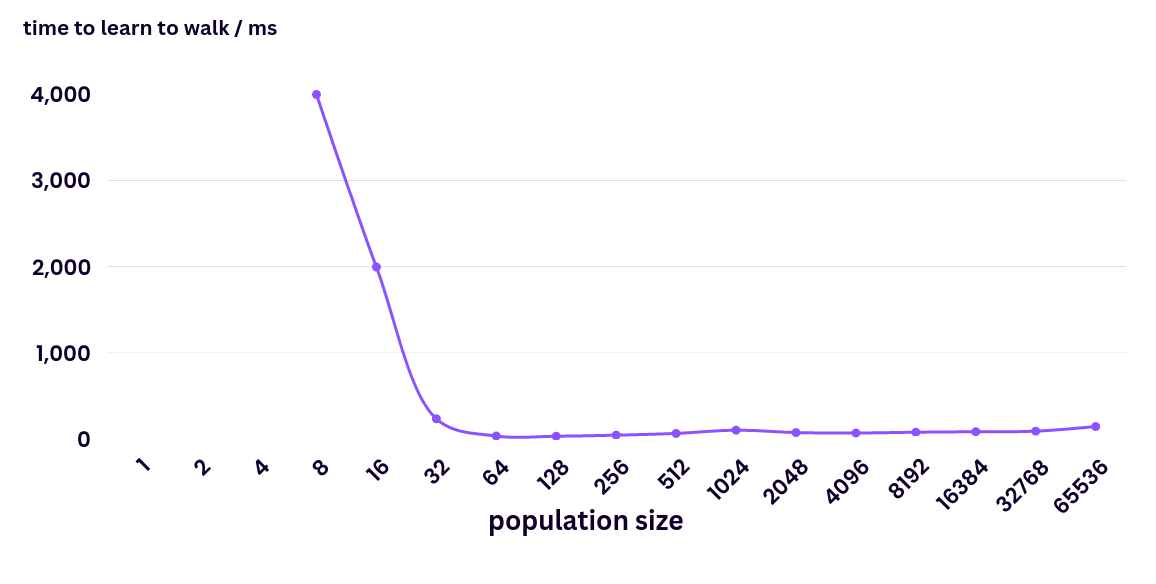
\includegraphics[width=3in]{resources/timetolearntowalk.png}
Illustration of advantage of using GPU's to simulate physics and run creature learning.

#if 0
\begin{figure}[H]
    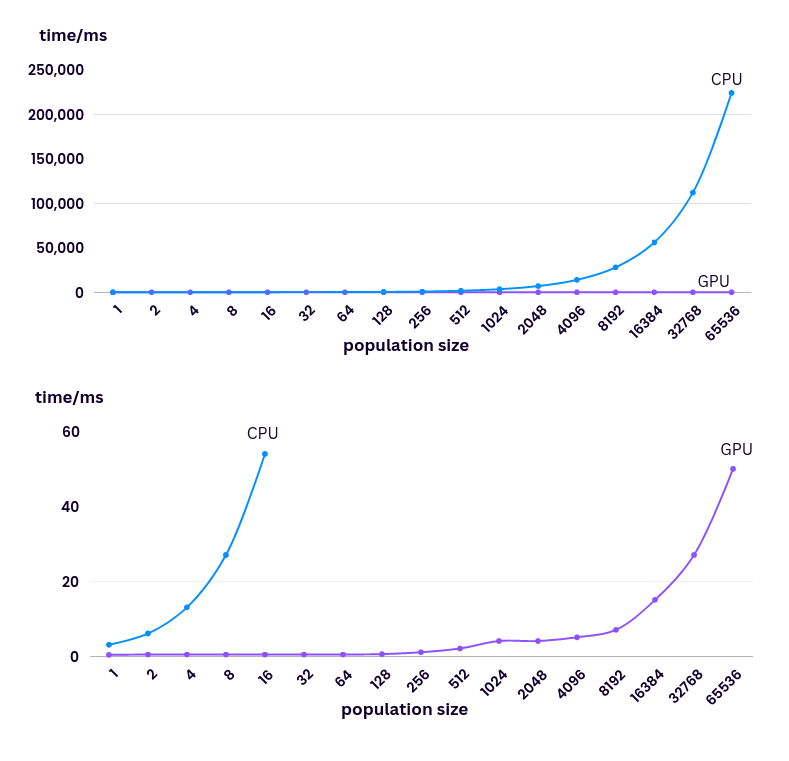
\includegraphics[width=3in]{popsizetime.png} %veličina u odnosu na širinu linije
    \caption{GPU vs CPU time per 1 episode step for different population sizes. GPU is running a program written in GLSL and CPU in Python. It can be seen that the CPU time grows much more quickly.}
    \label{fig:struktura} %label mora biti drugaciji za svaku sliku
\end{figure}

\begin{figure}[H]
    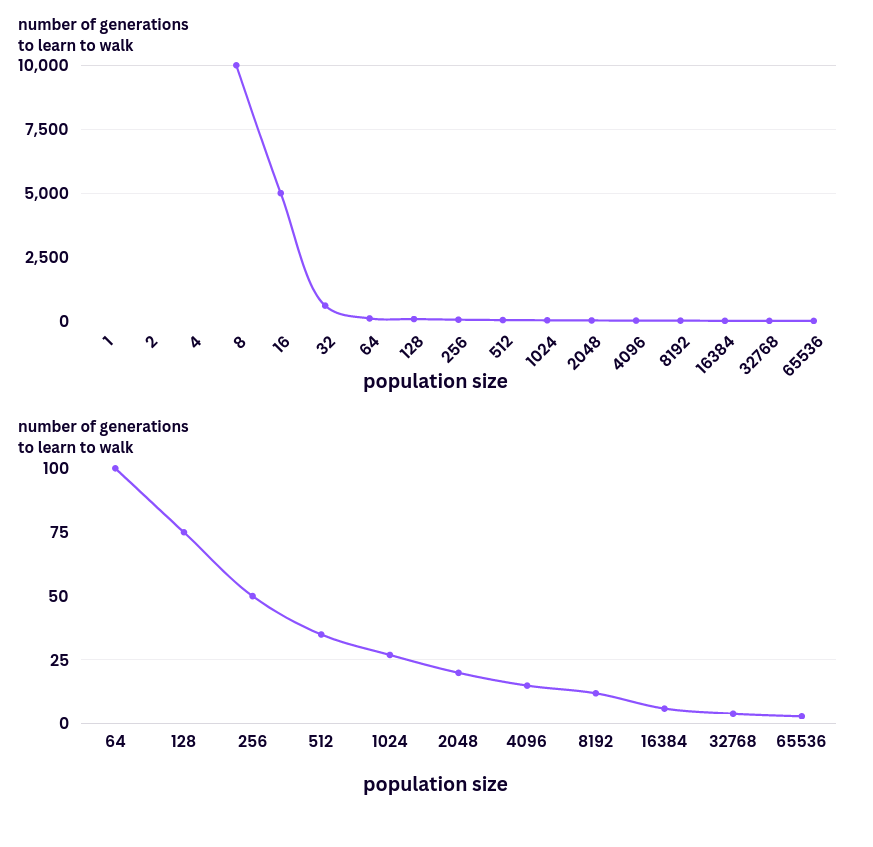
\includegraphics[width=3in]{numberofgenerationstolearntowalk.png} %veličina u odnosu na širinu linije
    \caption{As the population size grows number of generations to learn to walk falls. This is because when the population size is large, the probability that any creature is walking by pure chance is high.}
    \label{fig:struktura} %label mora biti drugaciji za svaku sliku
\end{figure}

\begin{figure}[H]
    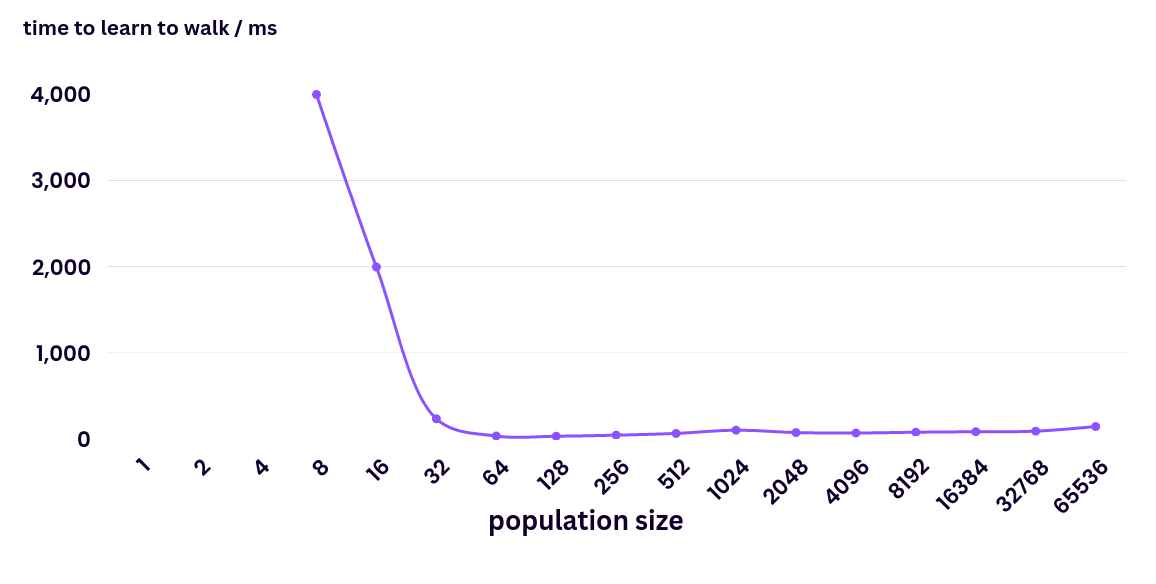
\includegraphics[width=3in]{resources/timetolearntowalk.png} %veličina u odnosu na širinu linije
    \caption{Illustration of advantage of using GPU's to simulate physics and run creature learning.}
    \label{fig:struktura} %label mora biti drugaciji za svaku sliku
\end{figure}
#endif